\documentclass[10pt,showpacs,preprintnumbers,footinbib,amsmath,amssymb,aps,prl,twocolumn,groupedaddress,superscriptaddress,showkeys]{revtex4-1}
\usepackage{graphicx}
\usepackage{dcolumn}
\usepackage{bm}
\usepackage[colorlinks=true,urlcolor=blue,citecolor=blue]{hyperref}
\usepackage{color}
\usepackage{listings}

\lstset{ %
  basicstyle=\footnotesize,        % the size of the fonts that are used for the code
  breakatwhitespace=false,         % sets if automatic breaks should only happen at whitespace
  breaklines=true,                 % sets automatic line breaking
  captionpos=t,                    % sets the caption-position to bottom
  deletekeywords={...},            % if you want to delete keywords from the given language
  escapeinside={\%*}{*)},          % if you want to add LaTeX within your code
  extendedchars=true,              % lets you use non-ASCII characters; for 8-bits encodings only, does not work with UTF-8
  frame=single,                    % adds a frame around the code
  keepspaces=true,                 % keeps spaces in text, useful for keeping indentation of code (possibly needs columns=flexible)
 % language=Python,                 % the language of the code
  morekeywords={*,...},           % if you want to add more keywords to the set
  numbers=left,                    % where to put the line-numbers; possible values are (none, left, right)
  numbersep=5pt,                   % how far the line-numbers are from the code
  showspaces=false,                % show spaces everywhere adding particular underscores; it overrides 'showstringspaces'
  showstringspaces=false,          % underline spaces within strings only
  showtabs=false,                  % show tabs within strings adding particular underscores
  stepnumber=1,                    % the step between two line-numbers. If it's 1, each line will be numbered
  tabsize=2,                       % sets default tabsize to 2 spaces
}


\begin{document}
\title{FYS3150 Computational Physics - Project 2}
\author{Nicholas Karlsen}

\begin{abstract}
  A look on the Jacobi Eigenvalue algorithm, and its application to a small selection of physical problems. Finding how the computation time of the algorithm develops by increasing the size of the problem, and how the implementation of the algorithm can make it more efficient. Found that the algorithm replicates analytical results to a reasonable degree of precision, and that it can be very easily applied to a large range of problems.
\end{abstract}

\maketitle

\section{Introduction}
  In this report, i will look closer at, and implement the Jacobi eigenvalue algorithm, used to solve eigenvalue problems in the form
  \begin{equation}
    A\mathbf v = \lambda \mathbf v
  \end{equation}
  where $A$ is a $N\times N$ matrix, $v\in \mathbb R^N$ a vector and $\lambda \in \mathbb R$ a scalar. Problems in this form shows up frequently in many areas of Physics, particularly in Quantum Mechanics, and in this report i will use the algorithm to solve 3 such problems using the algorithm, and see how it matches up with analytical results where applicable.

  My implementations of the algorithm discussed in this report can be found on my Github: \url{https://github.com/nicholaskarlsen/FYS3150}

\section{Theory, Algorithms and Methods}
  \subsection{Preservation of scalar product \& orthogonality in unitary transformations\label{subsec:preservation}}
    Consider an orthonormal set of basis vectors $\mathbf v_i$ such that $\mathbf v_j^T \mathbf v_i = \delta_{ij}$. Let unitary matrix $U$ where $U^T U= I_N$, where $I_N$ denotes the $N\times N$ identity matrix, operate on $\mathbf v_i$ to get $\mathbf w_i$
    \begin{equation}
      \mathbf w_i = U \mathbf v_i
    \end{equation}
    Then
    \begin{equation}
      \mathbf w_j^T\mathbf w_i = (U\mathbf v_j)^TU\mathbf v_i = \mathbf v_j^T U^T U \mathbf v_i
      = \mathbf v_j^T \mathbf v_i = \delta_{ij}
    \end{equation}
    In the unitary transformation of $\mathbf v_i$ both the scalar product and orthogonality has been preserved.

\subsection{Givens rotation}
  A Givens rotation is a unitary transformation which performs a rotation in the plane spanned by two coordinate axes, represented by the matrix in Eqn. \ref{eqn:givens}.
  \begin{equation}
    \label{eqn:givens}
    G(i, j, \theta) = 
    \begin{bmatrix}
      1 & \dots & 0 & \dots & 0 & \dots & 0 \\
      \vdots & \ddots & \vdots & & \vdots & & \vdots \\
      0 &\dots & \cos\theta & \dots  & - \sin \theta & \dots & 0 \\
      \vdots && \vdots & \ddots & \vdots && \vdots \\
      0 & \dots & \sin \theta & \dots & \cos \theta & \dots & 0 \\
      \vdots && \vdots && \vdots & \ddots & \vdots \\
      0 & \dots & 0 & \dots & 0 & \dots & 1
    \end{bmatrix}
  \end{equation}
  where nonzero entries $g_{kk}=1$ for $k\neq i,j$, $g_{kk}=cos\theta$ for $k=i,j$ and $g_{ji} = -g_{ij} = -\sin \theta$ \cite{givens}

  As the Givens transformation it unitary, it also follows that it preserves both the scalar product and orthogonality, as shown in the section prior.

\subsection{Jacobi Eigenvalue Algorithm \label{subsec:jacobi_algo}}
    The jacobi eigenvalue algorithm finds the eigenpairs of real, symmetric matrices by diagonalization with Givens rotation matrix repeatedly to produce similar matrices until the matrix becomes diagonal. By applying the same transformation to an orthogonal basis which spans the matrix, one also gets the associated eigenvectors to the eigenvalues once the matrix has been diagonalized.

    Each transformation, $G^T A G = B$, where $A, B$ are the symmetric matrices and $G$ is Givens matrix, can be summarized by the following changes in values when $A \rightarrow B$

    \begin{align}
      \begin{split}
      &\left.
      \begin{matrix}
        b_{ii} = a_{ii}            \\
        b_{ik} = a_{ik}c - a_{il}s \\
        b_{il} = a_{il}c + a_{ik}s            \\
      \end{matrix} \right\}
       \quad \textup{for } i\neq k, i\neq l \\
       &b_{kk} = a_{kk}c^2 - 2a_{kl}cs + a_{ll}s^2 \\
       &b_{ll} = a_{ll}c^2 + a_{kl}cs + a_{kk}s^2 \\
       &b_{kl} = (a_{kk} - a_{ll})cs + a_{kl}(c^2 - s^2)
      \end{split}
    \end{align}
    Where $c = \cos \theta, s = \sin \theta$. However, one can not know the rotation angle needed to diagonalize the matrix beforehand, so instead, the largest squared, non-diagonal entry is chosen and set to zero, and the rest of the matrix is rotated accordingly.

    By imposing that $b_{kl}=0$, it follows that $(a_{kk} - a_{ll})cs + a_{kl}(c^2 - s^2) = 0$. If $a_{kl}=0$, then $c=1$ and $s=0$.

    Next, $\tan \theta = t = s/c$ is obtained by defining
    \begin{equation}
      \tau = \frac{a_{ll} - a_{kk}}{2a_{kl}}
    \end{equation}
    And solving the quadratic equation $t^2 + 2\tau t - 1 = 0$, which has two solutions.
    \begin{equation}
      t = - \tau \pm \sqrt{1 + \tau^2}
    \end{equation}
    Which gives the $s, c$ in terms of $t$
    \begin{equation}
      c = \frac{1}{\sqrt{1 + t^2}}, \quad s = tc
    \end{equation}

   or written out in pseudocode; 
\begin{lstlisting}[mathescape=true, language=python, title=Jacobi Eigenvalue Algorithm]
$\tau = \frac{a_{ll} - a_{kk}}{2a_{kl}}$

if $\tau \geq 0$:
    $t = \frac{1}{\tau + \sqrt{1 + \tau^2}}$
else:
    $t = \frac{-1}{-\tau + \sqrt{1 + \tau^2}}$

$c = \frac{1}{\sqrt{1 + t^2}}$
$s = tc$

$a_{kk}' = a_{kk}$
$a_{ll}' = a_{ll}$

$a_{kk} = c^2 * a_{kk}' - 2cs * a_{kl} + s^2 * a_{ll}'$
$a_{ll} = s^2 * a_{kk}' + 2cs * a_{kl} + c^2 * a_{ll}'$
$a_{kl} = 0.0 $
$a_{lk} = 0.0 $

for $i = 1, 2, \dots N$:
    if $i \neq k$ and $i \neq l$:
        $a_{ik} = a_{ik} $
        $a_{il} = a_{il} $
        $a_{ik} = c * a_{ik} - s * a_{il} $
        $a_{ki} = a_{ik} $
        $a_{il} = c * a_{il} + s * a_{ik} $
        $a_{li} = a_{il} $
\end{lstlisting}

Which is repeated, until the largest squared off-diagonal element is less than some small tolerance, $a_{ij}^2 \leq \epsilon, i\neq j$, and the diagonal is populated by the eigenvalues.

\subsection{Some eigenvalue problems in Physics}
  \subsubsection{Buckling beam}
    A buckling beam, that is a flexible beam with length $L$ fixed on both sides and compressed can be modeled by the differential equation 
    \begin{equation}
      \gamma \frac{d^2}{dx^2}u(x) = -Fu(x)
    \end{equation}
    Where $u(x)$ denotes the vertical displacement of the beam at point $x \in [0, L]$, $F$ is the force due to the compression and $\gamma$ is a constant which contains information about the properties of the beam. The latter two are treated as constants, and because the beam is fixed on both ends, Dirichlet boundary conditions are applied such that, $u(0) = u(L) = 0$.

    By scaling $x$ such that $\rho = x / L$, and approximating the 2nd order derivative of $u(\rho)$ as a Taylor series, the problem can be discretized.
    \begin{equation}
      \frac{d^2}{dx^2} u(\rho) = \frac{u(\rho + h) - 2u(\rho) + u(\rho - h)}{h} + \mathcal O(h^2)
    \end{equation}
    Where $h$ denotes the discrete step size. By defining $\lambda = FL^2 / R$ and rewriting the problem as a linear algebra problem, we get

    \begin{equation}
      \label{eqn:eigenval matrix}
      \begin{bmatrix}
        d & e & 0 & \dots & 0 \\
        e & d & e &  & 0 \\
        \vdots & e & \ddots & \ddots & \vdots \\
        \vdots &  & \ddots & \ddots & e \\
        0 & \dots & \dots &  e & d
      \end{bmatrix}
      \begin{bmatrix}
        u_1 \\ u_2 \\ \vdots \\ \vdots \\ u_{N-1}
      \end{bmatrix}
      =
      \lambda
      \begin{bmatrix}
        u_1 \\ u_2 \\ \vdots \\ \vdots \\ u_{N-1}
      \end{bmatrix}
    \end{equation}

    Where $d=2/h^2$, $e=-1/h^2$.
    Which more specifically, is an eigenvalue problem. As such, this system can then be solved
    using the Jacobi Eigenvalue Algorithm. \cite{question_text}

    This problem in particular also has analytical eigenvalues, given by
    \begin{equation}
      \label{eqn:analytic eigenvals}
      \lambda_j = d + 2e\cos\left( \frac{j\pi}{N+1} \right), \quad j=1, 2, \dots, N
    \end{equation}


  \subsubsection{Quantum dots in three dimensions}
    Under the assumption of spherical symmetry, the radial part of the Schroedinger equation for one electron takes 
    the following form.
    \begin{equation}
      \label{eqn:radialschrodinger}
      -\frac{\hbar^2}{2m}\left( \frac{1}{r^2}\frac{d}{dr}r^2\frac{d}{dr} - \frac{l(l+1)}{r^2} \right)
      R(r) + V(r)R(r) = ER(r)
    \end{equation}
    In this case, we will let the potential, $V(r)=\frac{1}{2}kr^2, k=m\omega^2$, the Harmonic Oscillator potential.
    For more details on this, refer to Griffith's \cite{griffiths}, or another book on Quantum mechanics.

    Like the buckling beam, solutions to this problem can also be discretized and solved numerically as an eigenvalue
    problem.

    First, the system is scaled such that $\rho = r/\alpha,\enspace \rho \in [0, \infty)$, then set $l=0$, then Eqn. \ref{eqn:radialschrodinger} can be rewritten so that it takes the following form \cite{question_text}

    \begin{equation}
      \label{eqn:1electron_para}
      -\frac{d^2}{d\rho^2} u(\rho) + \rho^2 u(\rho) = \lambda u(\rho)
    \end{equation}
    Where $\lambda = 2m\alpha^2E /\hbar^2$ and $\alpha$ is fixed such that $mk\alpha^4/\hbar^2=1$.

    Which then results in the eigenvalue problem similar to Eqn. \ref{eqn:eigenval matrix}, but with non-constant entries along the diagonal. 
    \begin{equation}
      d_i = \frac{2}{h^2} + V_i, \quad V_i = \rho^2
    \end{equation}

    Similarly, two electrons in a harmonic oscillator which interact by coulomb repulsion can also be solved in a similar fashion, and written in the form

    \begin{equation}
      \label{eqn:2electron_para}
      -\frac{d^2}{d\rho^2} \psi(\rho) + \omega_r^2 \rho^2 \psi(\rho) + \frac{1}{\rho} = \lambda \psi(\rho)
    \end{equation}
    Where $\rho=r/\alpha$, $r$ this time denoting $|\vec r_1 - \vec r_2|$, the separation between the two electrons 
    and $\omega_r^2=mk\alpha^4/4\hbar^2$, is a constant that can be interpreted as the strength of the H.O potential.

    But again, i refer to \cite{question_text} for the full derivation.

    The alteration to Eqn. \ref{eqn:eigenval matrix} in order to model this problem is very similar to the 1 electron case, in that the potential is added to the diagonal elements, which now becomes

    \begin{equation}
      d_i = \frac{2}{h^2} + \omega_r^2 \rho^2
    \end{equation}
\section{Results and Discussions}
  The Jacobi eigenvalue solver that i wrote, found on my github as \lstinline{Project_2/code/jacobi_eigensolver.py}.
  In order to ensure that it was performing according to my expectations, i imposed the following unit tests
  \begin{enumerate}
    \item The computed eigenvalues match up with a tested, known solver. In this case, numpy.
    \item The orthonormality of the starting basis is retained in the resultant eigenvectors
  \end{enumerate}

  The function which finds the maximum of the squared non diagonal elements was also tested to work, and the function which constructs the matrix (See Eqn. \ref{eqn:eigenval matrix}) was found to produce a set of eigenvalues which match up with the analytical eigenvalues computed by Eqn. \ref{eqn:analytic eigenvals}.

  As such, under these conditions my implementation of the Jacobi eigensolver is working as expected.

  For benchmarking, i present Figures \ref{fig:time}, \ref{fig:count}, which in their limited range seems to imply that the number of iterations needed for convergence rises with $\mathcal O(N^2)$, and the time required $\approx \mathcal O(N)$, if we look away from $N\lessapprox 10^2$, which takes $>1s$. In these cases, factors not necessarily related to the algorithm itself may come into play, and the timings may be affected as such. How these trends evolve for $N>10^3$ may not follow the same pattern, and solving for these larger systems is not possible for me as of right now due to time constraints. It is also worth to note, that prior to adding Just-in-time compilation to my program, solving for $N=100$ took $\approx 40s$ on my computer, meaning that simply adding the jit decorator to my code increased performance by $\approx 400\%$, showing just how slow a dynamically interpreted language like python is at recursion.

  \begin{figure}[h!]
    \center
    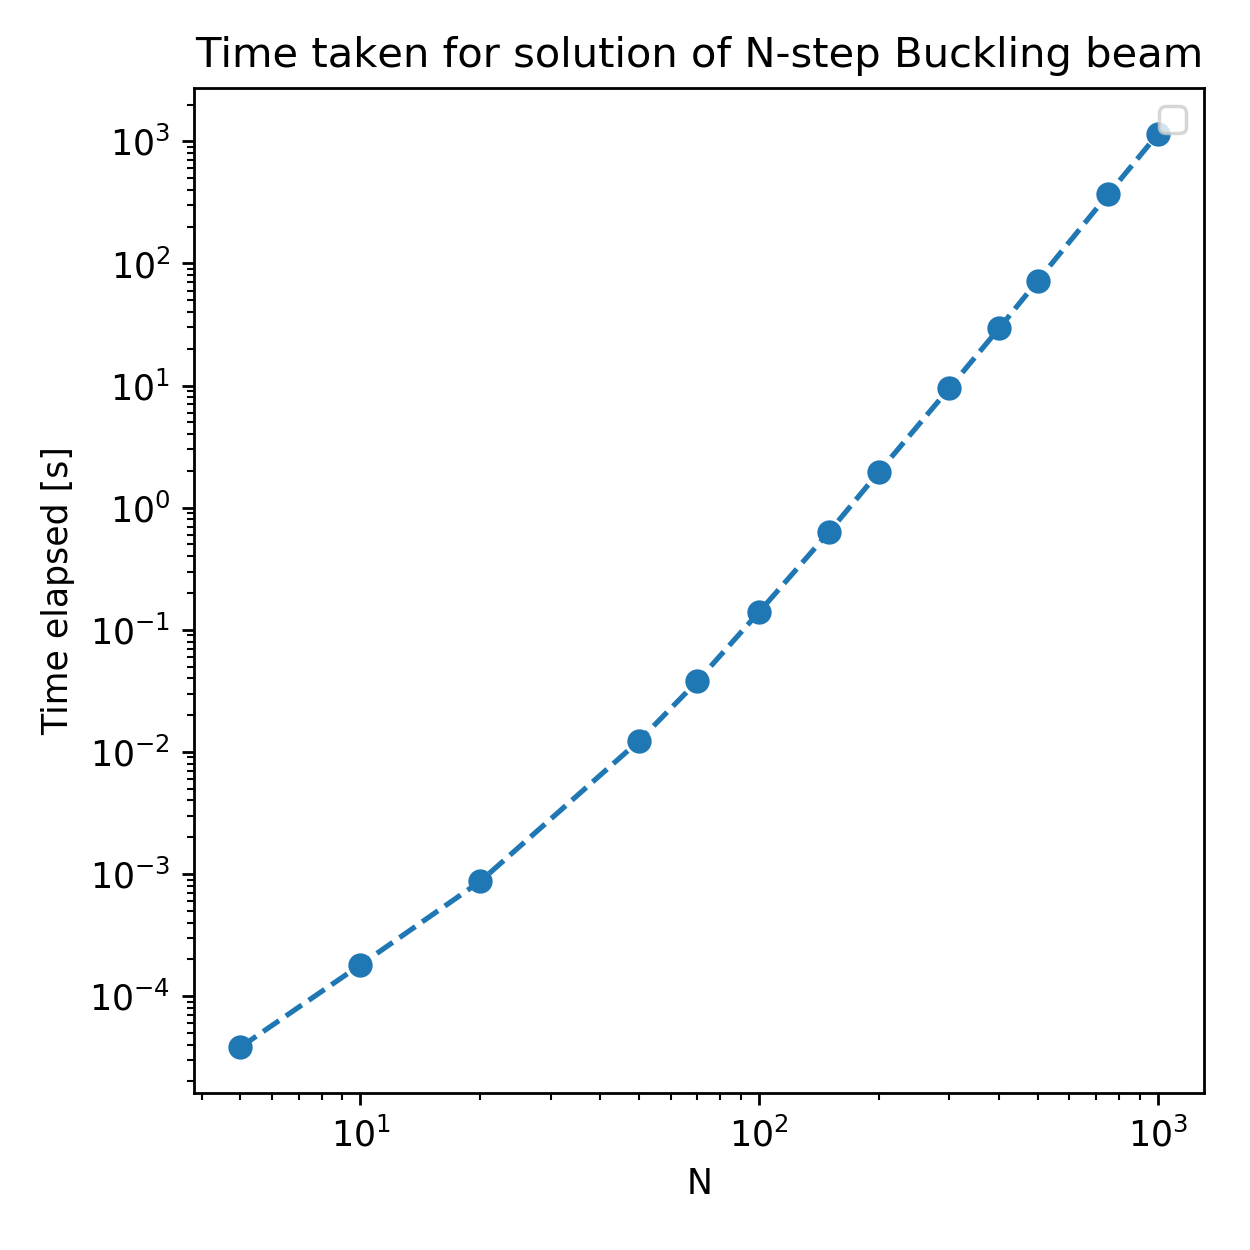
\includegraphics[width=8cm]{figs/q2c_timeloglog.png}
    \caption{Time taken for Jacobi eigenvalue solver to solve the buckling beam system for different N}
    \label{fig:time}
  \end{figure}

  \begin{figure}[h!]
    \center
    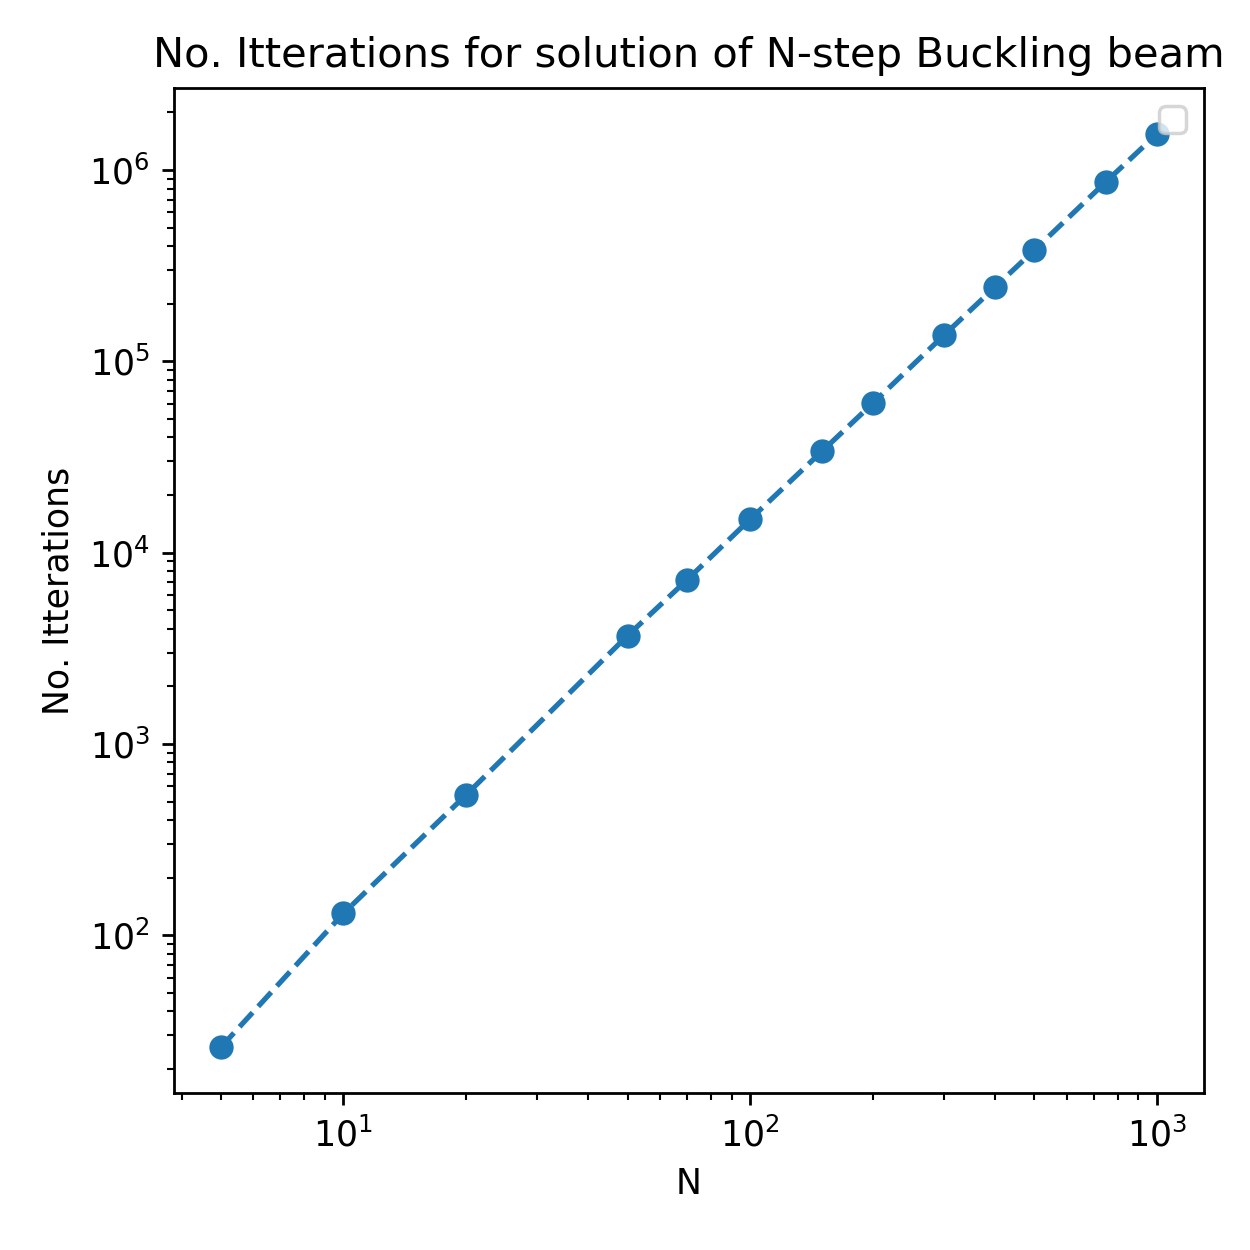
\includegraphics[width=8cm]{figs/q2c_countloglog.png}
    \caption{Number of iterations needed for Jacobi eigenvalue solver to solve the buckling beam system for different N}
    \label{fig:count}
  \end{figure}

  \begin{figure}[h!]
    \center
    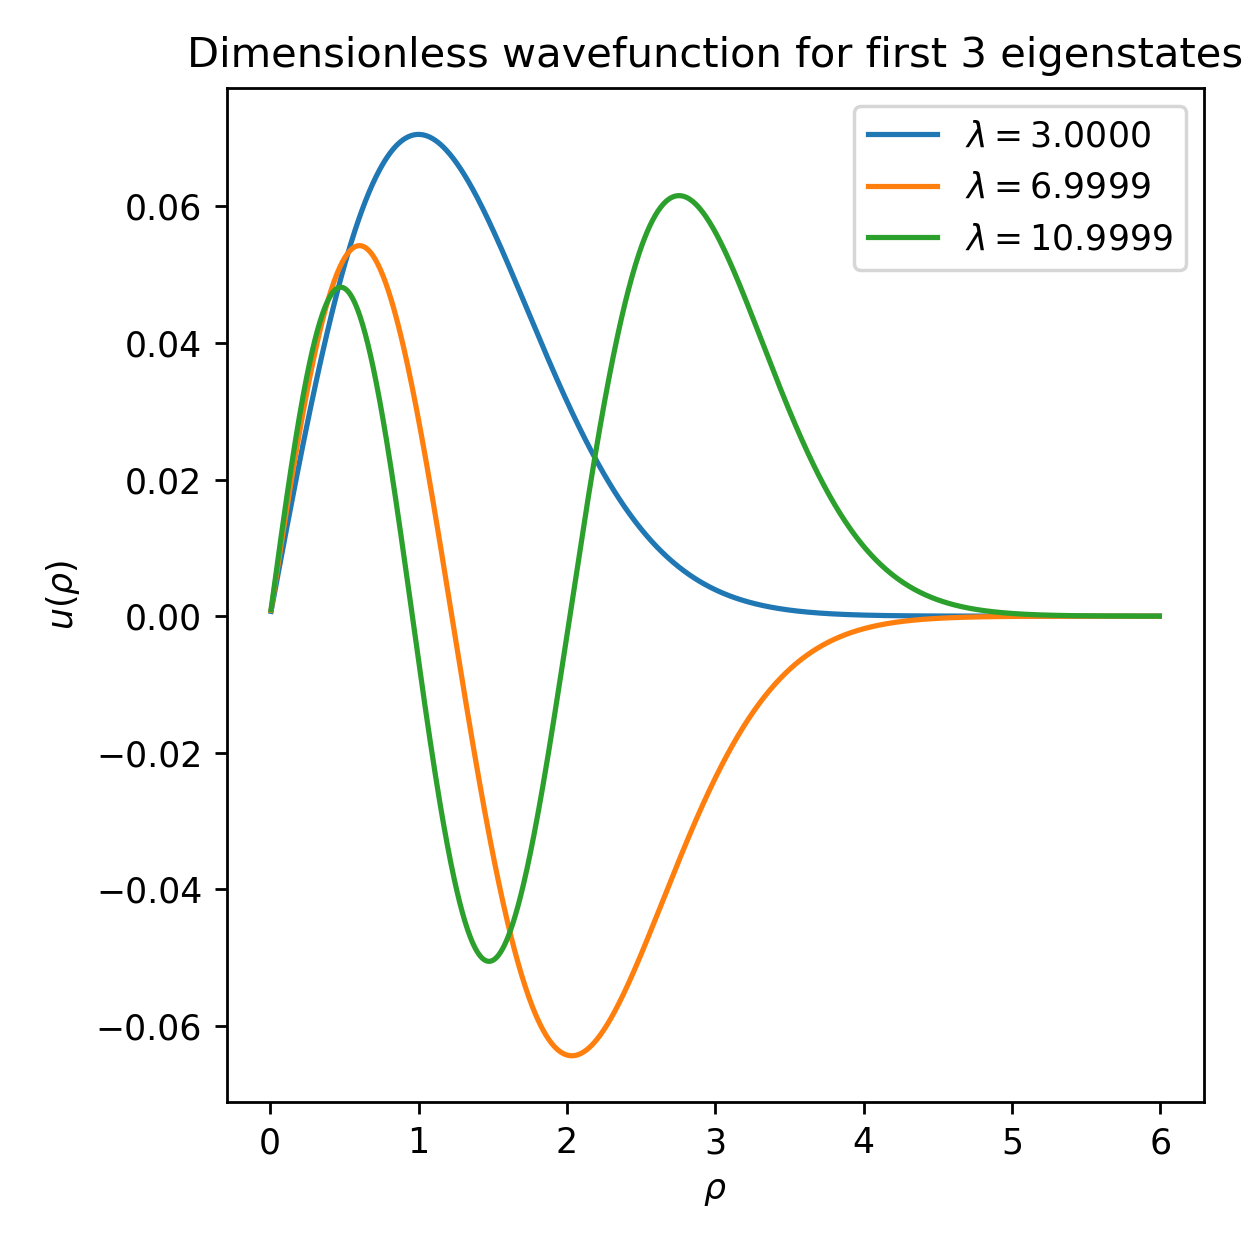
\includegraphics[width=8cm]{figs/question2d1000.png}
    \caption{First 3 eigenpairs in the solution of the harmonic oscillator potential for $N=1000$, requiring 1386366 transformations.}
    \label{fig:1electron}
  \end{figure}
  
  \begin{figure}[h!]
    \center
    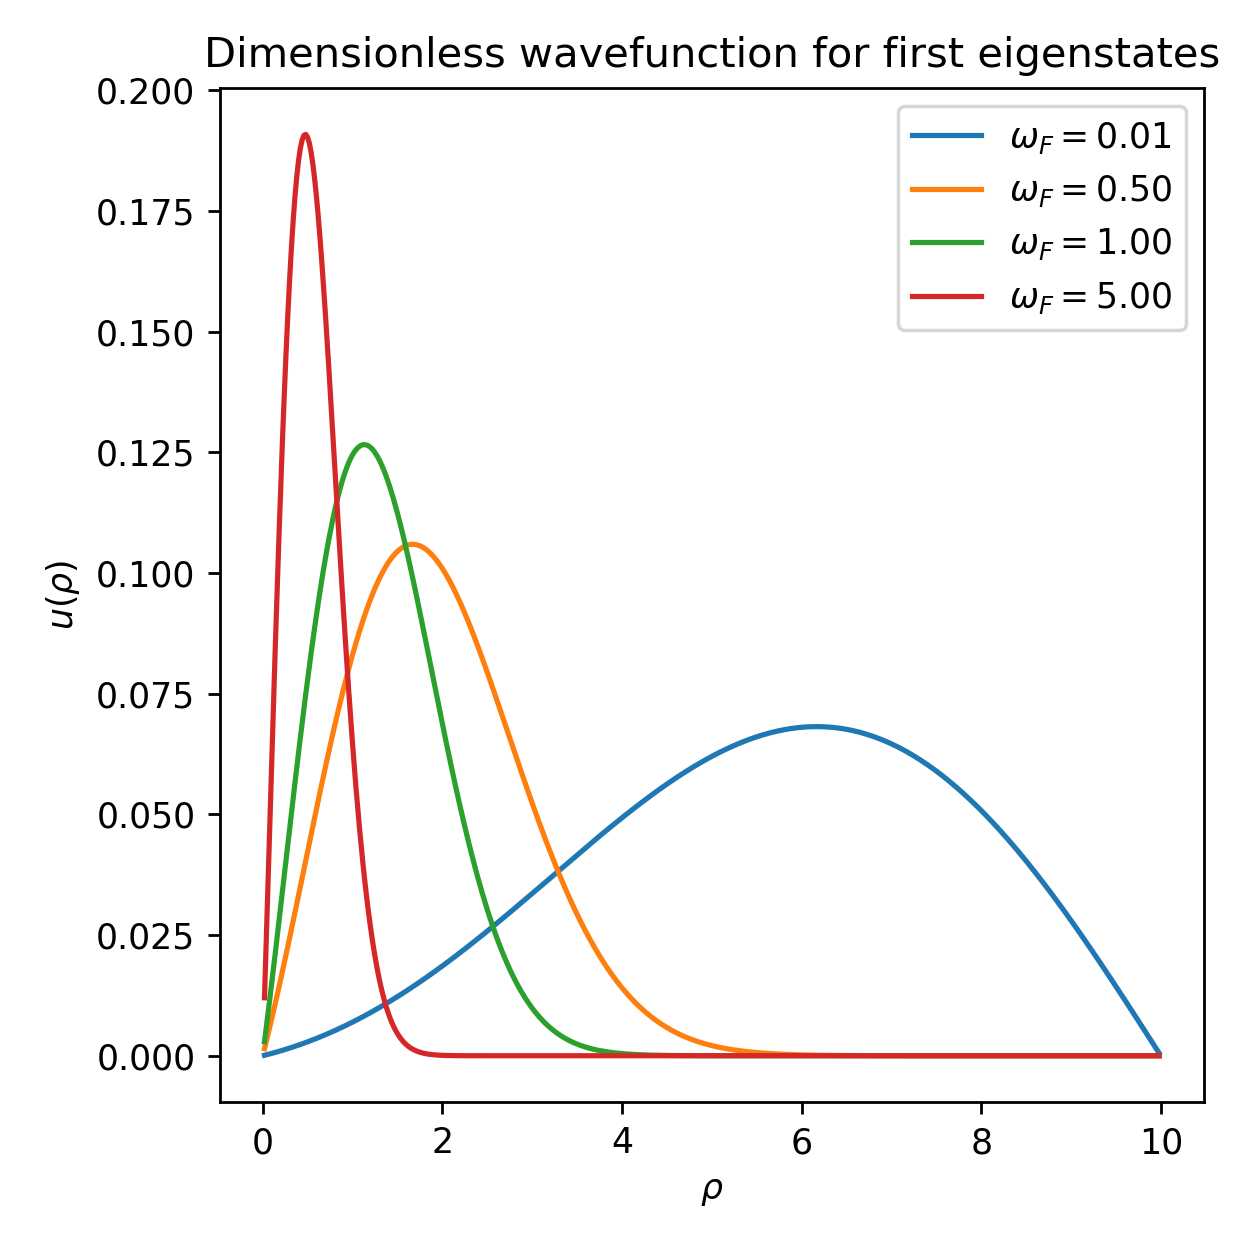
\includegraphics[width=8cm]{figs/question2e.png}
    \caption{Solution of the two electron problem in the lowest energy state for various $\omega_r$}
    \label{fig:2electrons}
  \end{figure}

  The algorithm was then used to solve the quantum mechanics problems outlined briefly in the theory section, which is kept in its scaled and parametrized form for the purposes of this report, as i am mostly interested in the behavior of the systems, and not the physical numbers.
  
  The data presented in Fig. \ref{fig:1electron} correlates to Eqn. \ref{eqn:1electron_para}, the radial component of a single electron in a harmonic oscillator potential. The expected first 3 eigenvalues for this system are: $\lambda = 3, 7, 11$ which my solver produced to just under four leading digits in a $\textup{dim}=1000$ solution. This accuracy, took $\sim 16$ minutes of computation on my computer.

  The the lowest eigenstate solution to the 2-electron problem is presented in Fig. \ref{fig:2electrons} for different $\omega_r$, which is representative of the strength of the harmonic oscillator potential. $\rho$ in this case, is to be interpreted as the separation between the two electrons, and $u(\rho)$ the relative probability of the electrons being separated by $\rho$. As we can see, by increasing $\omega_r$, the curves become narrower, and closes in on $0$. Physically, this translates to the average separation of the electrons becoming smaller, which means that the strength of the potential well is negating the effects of the repulsive coulomb force. Further, the possible spread of values become much sharper as $\omega_r$ increases.

\section{Conclusions}
  Have seen that the Jacobi Eigenvalue algorithm is applicable to a range of different physical systems by the clever use of scaling and parametrization, where it produces several possible solutions to the problem rather than just a very specific one, as you would get if you were to solve the problems as a standard differential equation. Further, i take a particular note of the massive performance increase yielded by introducing JIT compilation to the program and consider the potential speedups that may come from rewriting the program in a efficient, compiled language like FORTRAN or C++, which could enable me to look at even bigger problems (within reasonable computation time).
  Have also discovered the immense benefit of applying unit tests where possible, as it greatly reduced overall development time by allowing me to determine the functionality of the individual functions in my program as i wrote them.

  Lastly, take particular note of how flexible this algorithm can be, for solving a range of physical problem. For quantum mechanical problems in particular, if the problem can be reduced to a 1-D problem, the algorithm can be used to solve for many different potentials, requiring only minor adjustments diagonal of the initial matrix (Eqn. \ref{eqn:eigenval matrix}).


\begin{thebibliography}{99}
\bibitem{lecture_notes} M.~Hjorth-Jensen, Computational Physics - Lecture Notes 2015, (2015).
\bibitem{givens} Wikipedia contributors, Givens rotation --- {Wikipedia}{,} The Free Encyclopedia, [Online; accessed 1-October-2018]
\bibitem{question_text} M,~Hjorth-Jensen, Eigenvalue problems, from the equations of a buckling beam
to Schroedinger’s equation for two electrons in a three-
dimensional harmonic oscillator well - Project 2 (2018)
\bibitem{griffiths} D. J. Griffiths, Introduction to Quantum Mechanics 2nd Edition, (2004)
\end{thebibliography}

\end{document}  